\documentclass{article}
\usepackage{amsmath}
\usepackage{amssymb}
\usepackage[pdftex]{graphicx}
\usepackage[]{mcode}

\pdfpagewidth 8.5in
\pdfpageheight 11in
\topmargin -1in
\headheight 0in
\headsep 0in
\textheight 8.5in
\textwidth 6.5in
\oddsidemargin 0in
\evensidemargin 0in
\headheight 50pt
\headsep 0in
\footskip .75in

\title{STA 601 - Lab 1}
\author{Kedar Prabhudesai}
\date{September 6, 2013}

\begin{document}
\maketitle

\noindent {\Large\underline{\textbf{Beta-Binomial Model:}}}\\

\noindent Likelihood function: $y|\theta \sim \binom{n}{y}\right\theta^y(1-\theta)^{n-y}$\\

\noindent Prior: $\theta \sim Beta(a,b).$\\

\noindent Posterior: $\theta|y \sim Beta(a+y,b+n-y)$\\

\begin{enumerate}
\item Using \emph{Jeffrey's Prior} [$Beta(\frac{1}{2},\frac{1}{2})$] as default prior, the posterior distributions for probabilities of success are:\\
\begin{eqnarray*}
p_A \sim Beta(11.5,3.5)\\
p_B \sim Beta(5.5,1.5)\\
\end{eqnarray*}

\begin{center}
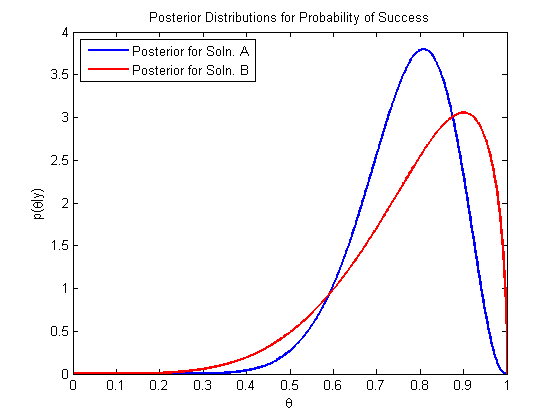
\includegraphics[scale=0.75]{postDists.png}
\end{center}

\item To find that the probability of success is at least 80\%, we can find the area under the posterior density to the right of $0.8$. This is equivalent
finding the $1-cdf(0.8)$ for each distribution. Hence we get,

\begin{eqnarray*}
P(p_A \ge 0.8) = 1 - P(p_A < 0.8) = 42.043790 \%\\
P(p_B \ge 0.8) = 1 - P(p_B < 0.8) = 53.546303 \%
\end{eqnarray*}

\item To truly determine if Solution B has higher success rate then Solution A, we can do a Monte-Carlo simulation
by drawing a large number ($100,000$) of random samples from the two posterior distributions. Then we can compare the proportion of samples from B greater than the ones from A. Doing so we get,

\begin{eqnarray*}
P(p_B > p_A) =  57.422000\%
\end{eqnarray*}

\item From these results we do see that Solution B is indeed performing better than Solution A. 

\end{enumerate}

\noindent {\Large\underline{\textbf{Appendix:}}}\\
\lstinputlisting{C:/Users/ksp6/Documents/Classes/2013-Fall/STA601-BayesAndModStats/labs/lab1/sta601_lab1_ksp6.m}

\end{document}